\documentclass{article}

\newif\ifanswers
\answerstrue % comment out to hide answers

\usepackage[compact]{titlesec}
\usepackage{fancyhdr} % Required for custom headers
\usepackage{lastpage} % Required to determine the last page for the footer
\usepackage{extramarks} % Required for headers and footers
\usepackage[usenames,dvipsnames]{color} % Required for custom colors
\usepackage{graphicx} % Required to insert images
\usepackage{listings} % Required for insertion of code
\usepackage{courier} % Required for the courier font
\usepackage{lipsum} % Used for inserting dummy 'Lorem ipsum' text into the template
\usepackage{enumerate}
\usepackage{enumitem}
\usepackage{subfigure}
\usepackage{booktabs}
\usepackage{amsmath, amsthm, amssymb}
\usepackage[maxbibnames=99,maxcitenames=1]{biblatex}
\usepackage{caption}
\usepackage{hyperref}
\captionsetup[table]{skip=4pt}
\usepackage{framed}
\usepackage{bm}
\usepackage{minted}
\usepackage{soul}
\usepackage[utf8]{vietnam}
\usepackage[vietnamese,english]{babel}

\graphicspath{{images/}}

\addbibresource{references.bib} %Import the bibliography file
\AtNextBibliography{\small}

\usepackage{tikz}
\usetikzlibrary{positioning, patterns, fit}


% Margins
\topmargin=-0.45in
\evensidemargin=0in
\oddsidemargin=0in
\textwidth=6.5in
\textheight=9.0in
\headsep=0.25in

\linespread{1.1} % Line spacing

% Set up the header and footer
\pagestyle{fancy}
\rhead{\hmwkAuthorName} % Top left header
\lhead{\hmwkClass: \hmwkTitle} % Top center head
\lfoot{\lastxmark} % Bottom left footer
\cfoot{} % Bottom center footer
\rfoot{Page\ \thepage\ of\ \protect\pageref{LastPage}} % Bottom right footer
\renewcommand\headrulewidth{0.4pt} % Size of the header rule
\renewcommand\footrulewidth{0.4pt} % Size of the footer rule

\setlength\parindent{0pt} % Removes all indentation from paragraphs

\newenvironment{answer}{
    % Uncomment this if using the template to write out your solutions.
    {\bf Answer:} \sf \begingroup\color{red}
}{\endgroup}%
%----------------------------------------------------------------------------------------
%	CODE INCLUSION CONFIGURATION
%----------------------------------------------------------------------------------------

\definecolor{MyDarkGreen}{rgb}{0.0,0.4,0.0} % This is the color used for comments
\definecolor{shadecolor}{gray}{0.9}

\lstloadlanguages{Python} % Load Perl syntax for listings, for a list of other languages supported see: ftp://ftp.tex.ac.uk/tex-archive/macros/latex/contrib/listings/listings.pdf
\lstset{language=Python, % Use Perl in this example
        frame=single, % Single frame around code
        basicstyle=\footnotesize\ttfamily, % Use small true type font
        keywordstyle=[1]\color{Blue}\bf, % Perl functions bold and blue
        keywordstyle=[2]\color{Purple}, % Perl function arguments purple
        keywordstyle=[3]\color{Blue}\underbar, % Custom functions underlined and blue
        identifierstyle=, % Nothing special about identifiers
        commentstyle=\usefont{T1}{pcr}{m}{sl}\color{MyDarkGreen}\small, % Comments small dark green courier font
        stringstyle=\color{Purple}, % Strings are purple
        showstringspaces=false, % Don't put marks in string spaces
        tabsize=5, % 5 spaces per tab
        %
        % Put standard Perl functions not included in the default language here
        morekeywords={rand},
        %
        % Put Perl function parameters here
        morekeywords=[2]{on, off, interp},
        %
        % Put user-defined functions here
        morekeywords=[3]{test},
       	%
        morecomment=[l][\color{Blue}]{...}, % Line continuation (...) like blue comment
        numbers=left, % Line numbers on left
        firstnumber=1, % Line numbers start with line 1
        numberstyle=\tiny\color{Blue}, % Line numbers are blue and small
        stepnumber=5 % Line numbers go in steps of 5
}

% Creates a new command to include a perl script, the first parameter is the filename of the script (without .pl), the second parameter is the caption
\newcommand{\perlscript}[2]{
\begin{itemize}
\item[]\lstinputlisting[caption=#2,label=#1]{#1.pl}
\end{itemize}
}

%----------------------------------------------------------------------------------------
%	NAME AND CLASS SECTION
%----------------------------------------------------------------------------------------

\newcommand{\hmwkTitle}{Homework 2} % Assignment title
\newcommand{\hmwkClass}{INT3404E 20 - Image Processing} % Course/class
\newcommand{\hmwkAuthorName}{Trần Phương Linh} % Your name

\newcommand{\ifans}[1]{\ifanswers \color{red} \vspace{5mm} \textbf{Solution: } #1 \color{black} \vspace{5mm} \fi}

% Chris' notes
\definecolor{CMpurple}{rgb}{0.6,0.18,0.64}
\newcommand\cm[1]{\textcolor{CMpurple}{\small\textsf{\bfseries CM\@: #1}}}
\newcommand\cmm[1]{\marginpar{\small\raggedright\textcolor{CMpurple}{\textsf{\bfseries CM\@: #1}}}}

%----------------------------------------------------------------------------------------
%	TITLE PAGE
%----------------------------------------------------------------------------------------
\title{
\vspace{-1in}
\textmd{\textbf{\hmwkClass:\ \hmwkTitle} \\ \hmwkAuthorName}\\
}
\author{}
% \date{\textit{\small Updated \today\ at \currenttime}} % Insert date here if you want it to appear below your name
\date{}

\setcounter{section}{0} % one-indexing
\begin{document}
\maketitle

\section{Ex1 - Image Filtering}
\subsection{Mã nguồn}
\subsubsection{padding\_img() function}
\begin{lstlisting}[caption={Code of padding\_img() function}, label={padding\_img}]
def padding_img(img, filter_size=3):
    pad_size = filter_size // 2
    padded_img = np.pad(img, pad_size, mode='edge')
    return padded_img
\end{lstlisting}

\begin{itemize}
    
    \item Thuật toán:
    \begin{itemize}
        \item Sử dụng hàm np.pad từ thư viện NumPy để thêm các hàng và cột vào xung quanh ảnh ban đầu. Tham số pad\_size được tính bằng cách chia filter\_size cho 2, và sau đó np.pad được sử dụng để thêm các hàng và cột tương ứng.
        \item Chế độ (mode) được đặt là 'edge', điều này có nghĩa là các giá trị pixel ở biên của ảnh sẽ được sao chép từ các hàng và cột cuối cùng của ảnh. Điều này giúp giữ nguyên các biên của ảnh và tránh tạo ra hiệu ứng không mong muốn khi đệm.
    \end{itemize}
\end{itemize}


\subsubsection{mean\_filter() function}
\begin{lstlisting}[caption={Code of mean\_filter() function}, label={mean\_filter()}]
def mean_filter(img, filter_size=3):
    # Perform padding
    padded_img = padding_img(img, filter_size)

    # Get image shape
    height, width = img.shape

    # Initialize smoothed image
    smoothed_img = np.zeros_like(img)

    # Apply mean filter
    for i in range(height):
        for j in range(width):
            # Extract neighborhood
            neighborhood = padded_img[i:i + filter_size, j:j + filter_size]
            # Apply mean filter
            smoothed_img[i, j] = np.mean(neighborhood)

    return smoothed_img
\end{lstlisting}

\begin{itemize}
    
    \item Thuật toán:
    \begin{itemize}
        \item Hình ảnh đầu vào được thêm viền bằng cách sử dụng hàm padding\_img, đảm bảo các pixel ở mép của hình ảnh cũng có thể được xử lý.
        \item Một ma trận có kích thước giống với hình ảnh đầu vào được khởi tạo để chứa hình ảnh được làm mịn.
        \item Hàm duyệt qua từng pixel của hình ảnh, và tại mỗi vị trí, trích xuất vùng lân cận xung quanh pixel đó bằng cách sử dụng kích thước bộ lọc.

        \item Bộ lọc trung bình được áp dụng bằng cách tính trung bình của các giá trị pixel trong vùng lân cận.
        \item Giá trị trung bình được gán cho pixel tương ứng trong hình ảnh được làm mịn.
   
    \end{itemize}
\end{itemize}



\subsubsection{median\_filter() function}
\begin{lstlisting}[caption={Code of median\_filter() function}, label={median\_filter()}]
def median_filter(img, filter_size=3):
    # Perform padding
    padded_img = padding_img(img, filter_size)

    # Get image shape
    height, width = img.shape

    # Initialize smoothed image
    smoothed_img = np.zeros_like(img)

    # Apply median filter
    for i in range(height):
        for j in range(width):
            # Extract neighborhood
            neighborhood = padded_img[i:i + filter_size, j:j + filter_size]
            # Apply median filter
            smoothed_img[i, j] = np.median(neighborhood)

    return smoothed_img
\end{lstlisting}

\begin{itemize}
    
    \item Thuật toán:
    \begin{itemize}
        \item Hình ảnh đầu vào được thêm viền bằng cách sử dụng hàm padding\_img, đảm bảo các pixel ở mép của hình ảnh cũng có thể được xử lý.
        \item Một ma trận có kích thước giống với hình ảnh đầu vào được khởi tạo để chứa hình ảnh được làm mịn.
        \item Hàm duyệt qua từng pixel của hình ảnh, và tại mỗi vị trí, trích xuất vùng lân cận xung quanh pixel đó bằng cách sử dụng kích thước bộ lọc.
        \item Bộ lọc trung vị được áp dụng bằng cách tính giá trị trung vị của các giá trị pixel trong vùng lân cận.
        \item Giá trị trung vị được gán cho pixel tương ứng trong hình ảnh được làm mịn.
    \end{itemize}
\end{itemize}


\subsubsection{psnr() function}
\begin{lstlisting}[caption={Code of psnr() function}, label={psnr()}]
def psnr(gt_img, smooth_img):
    # Calculate Mean Square Error (MSE)
    mse = np.mean((gt_img - smooth_img) ** 2)

    # Maximum possible pixel value
    max_pixel = 255

    # Calculate PSNR
    psnr_score = 10 * math.log10((max_pixel ** 2) / mse)

    return psnr_score
\end{lstlisting}

\begin{itemize}
    
    \item Thuật toán:
    \begin{itemize}
        \item Tính giá trị MSE (Mean Square Error) giữa ảnh gốc và ảnh đã lọc, sau đó sử dụng công thức PSNR đã cho để tính toán điểm số PSNR và trả về nó.
    \end{itemize}
\end{itemize}



\subsection{Output}
\subsubsection{Kết quả sau khi thực hiện bộ lọc mean filter}
\begin{itemize}
    \item Ảnh sau khi thực hiện bộ lọc mean filter:
\end{itemize}

\begin{figure}[H]
    \centering
    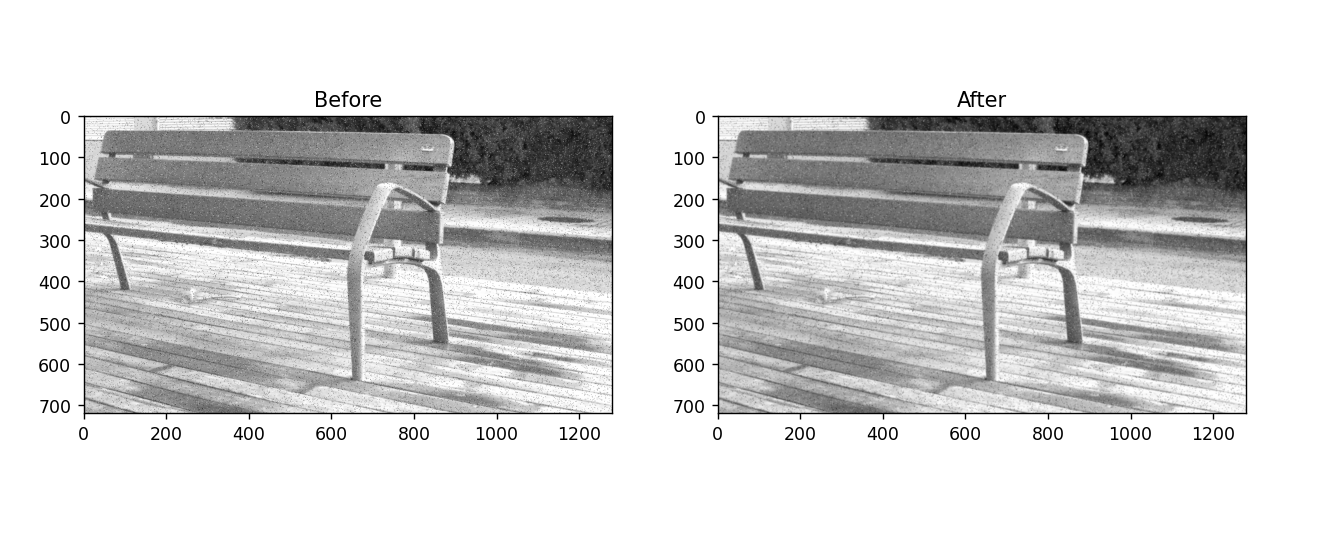
\includegraphics[width=0.75\textwidth]{before-after-mean}
    \caption{After mean filter}
    \label{before-after-mean}
\end{figure}

\begin{itemize}
    \item Giá trị PSNR score: \lstinline{31.61}
\end{itemize}

\subsubsection{Kết quả sau khi thực hiện bộ lọc median filter}
\begin{itemize}
    \item Ảnh sau khi thực hiện bộ lọc median filter:
\end{itemize}

\begin{figure}[H]
    \centering
    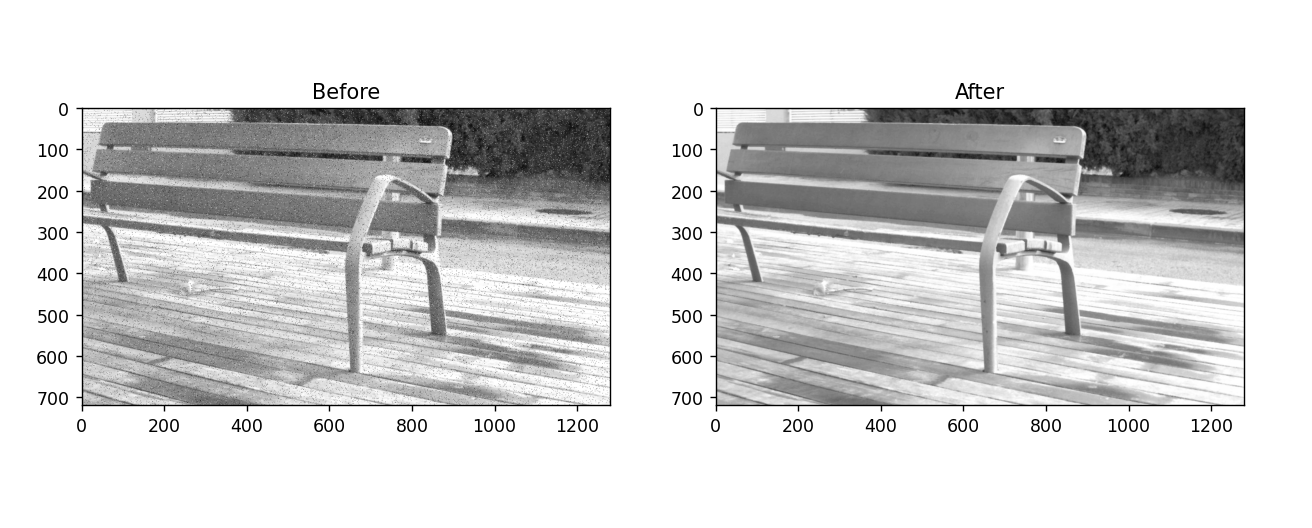
\includegraphics[width=0.75\textwidth]{before-after-median}
    \caption{After median filter}
    \label{before-after-median}
\end{figure}

\begin{itemize}
    \item Giá trị PSNR score: \lstinline{37.12}
\end{itemize}

\subsubsection{Nhận xét về PSNR score}

\begin{itemize}
    \item Dựa trên các chỉ số Peak Signal-to-Noise Ratio (PSNR) đã cung cấp:
    \begin{itemize}
        \item Điểm số PSNR của mean filter: 31.61
        \item Điểm số PSNR của median filter: 37.12
    \end{itemize}
    
    \item Điểm số PSNR đo lường chất lượng của ảnh sau khi lọc, trong đó giá trị PSNR cao hơn chỉ ra chất lượng ảnh tốt hơn. Trong trường hợp này, median filter có điểm số PSNR cao hơn đáng kể so với mean filter. Điều này ngụ ý rằng median filter có hiệu suất tốt hơn trong việc bảo tồn chất lượng hình ảnh và giảm nhiễu.
    \item Do đó, xét theo các chỉ số PSNR, median filter nên được chọn hơn mean filter cho các hình ảnh đã cung cấp.
    
\end{itemize}



\section{Ex 2.1 và Ex 2.2 - Fourier Transform}
\subsection{Mã nguồn}

\subsubsection{DFT\_slow() function}
\begin{lstlisting}[caption={Code of DFT\_slow() function}]
def DFT_slow(data):
    N = len(data)
    n = np.arange(N)
    k = n.reshape((N, 1))
    e = np.exp(-2j * np.pi * k * n / N)
    return np.dot(e, data)
\end{lstlisting}

\begin{itemize}
    \item Thuật toán:
    \begin{itemize}
        \item Xác định độ dài của dữ liệu đầu vào.
        \item Tạo một mảng numpy chứa các chỉ số từ 0 đến độ dài dữ liệu - 1.
        \item Tạo một ma trận exponents.
        \item Tính toán DFT bằng cách nhân ma trận exponents với dữ liệu đầu vào và trả về kết quả.
        
    \end{itemize}
\end{itemize}


\subsubsection{DFT\_2D() function}
\begin{lstlisting}[caption={Code of DFT\_2D() function}, label={DFT\_2D()}]
def DFT_2D(gray_img):
    row_fft = np.fft.fft(gray_img, axis=1)

    row_col_fft = np.fft.fft(row_fft, axis=0)

    return row_fft, row_col_fft
\end{lstlisting}

\begin{itemize}
    
    \item Thuật toán:
    \begin{itemize}
        \item Thực hiện biến đổi Fourier theo hàng cho mỗi hàng của hình ảnh đầu vào, sử dụng np.fft.fft với trục axis=1.
        \item Thực hiện biến đổi Fourier theo cột cho mỗi cột của kết quả từ bước trước, sử dụng np.fft.fft với trục axis=0.
    \end{itemize}
\end{itemize}



\subsection{Output}
\subsubsection{Kết quả sau khi thực hiện DFT\_2D() function}
\begin{itemize}
    \item Ảnh sau khi thực hiện DFT\_2D() function:
\end{itemize}

\begin{figure}[H]
    \centering
    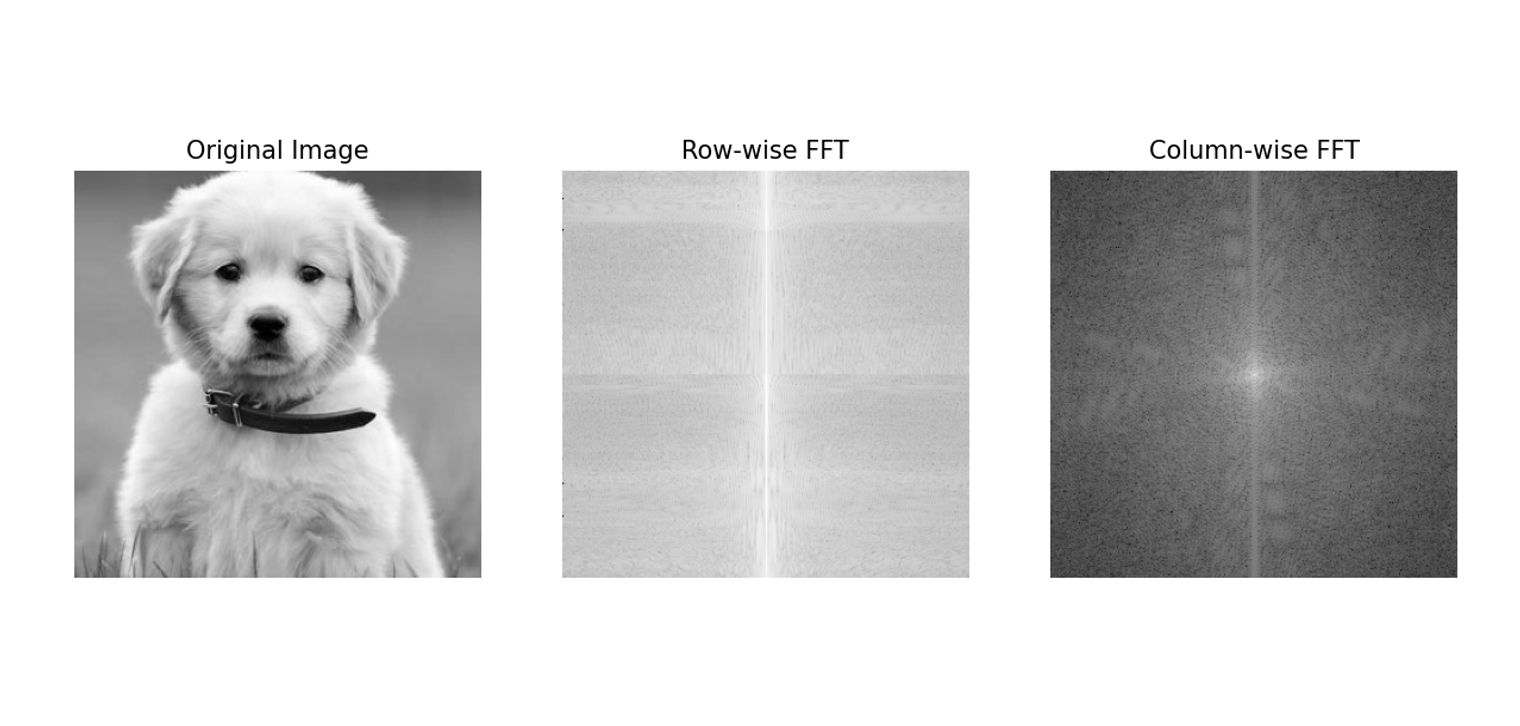
\includegraphics[width=0.75\textwidth]{ex212_output}
    \caption{After DFT\_2D() function}
    \label{ex212_output}
\end{figure}


\section{Ex 2.3 và Ex 2.4}
\subsection{Mã nguồn}
\subsubsection{filter\_frequency() function}
\begin{lstlisting}[caption={Code of filter\_frequency() function}, label={filter\_frequency()}]
def filter_frequency(orig_img, mask):
    # Fourier transform of the original image
    f_img = fft2(orig_img)

    # Shift frequency coefficients to center
    f_img_shifted = fftshift(f_img)

    # Apply mask in frequency domain
    f_img_filtered = f_img_shifted * mask

    # Shift frequency coefficients back
    f_img_filtered_shifted = ifftshift(f_img_filtered)

    # Inverse transform
    img = np.abs(ifft2(f_img_filtered_shifted))

    return f_img_filtered, img
\end{lstlisting}

\begin{itemize}
    
    \item Thuật toán:
    \begin{itemize}
        \item Biến đổi Fourier của hình ảnh gốc (orig\_img): Hình ảnh gốc được chuyển từ miền không gian sang miền tần số bằng cách sử dụng biến đổi Fourier (fft2), tạo ra một hình ảnh tần số (f\_img).
        \item Dịch các hệ số tần số về trung tâm: Các hệ số tần số của hình ảnh được dịch sang trung tâm bằng cách sử dụng hàm fftshift. Điều này cần thiết để chuẩn bị cho việc áp dụng mask.
        \item Áp dụng mask trong miền tần số: Mask được áp dụng trực tiếp lên hình ảnh tần số dịch chuyển (f\_img\_shifted). Mask này được ánh xạ pixel từ pixel tương ứng trên hình ảnh tần số.
        \item Dịch ngược các hệ số tần số: Sau khi áp dụng mask, các hệ số tần số được dịch trở lại vị trí ban đầu bằng cách sử dụng ifftshift
        \item Biến đổi nghịch: Cuối cùng, biến đổi Fourier nghịch (ifft2) được áp dụng để chuyển hình ảnh từ miền tần số trở lại miền không gian. Giá trị tuyệt đối của kết quả được lấy để đảm bảo giá trị thực.
    \end{itemize}
\end{itemize}


\subsubsection{create\_hybrid\_img() function}
\begin{lstlisting}[caption={Code of reate\_hybrid\_img() function}, label={reate\_hybrid\_img()}]
def create_hybrid_img(img1, img2, r):
    # Step 1: Fourier transform for two input images
    img1_fft = fft2(img1)
    img2_fft = fft2(img2)

    # Step 2: Shift the frequency coefficients to center using fftshift
    img1_fft_shifted = fftshift(img1_fft)
    img2_fft_shifted = fftshift(img2_fft)

    # Step 3: Create mask based on radius (r)
    rows, cols = img1.shape
    crow, ccol = rows // 2, cols // 2
    mask = np.zeros((rows, cols), dtype=np.float32)
    for i in range(rows):
        for j in range(cols):
            dist = np.sqrt((i - crow) ** 2 + (j - ccol) ** 2)
            if dist <= r:
                mask[i, j] = 1

    # Step 4: Combine frequencies of two images using mask
    img1_hybrid_fft = img1_fft_shifted * mask
    img2_hybrid_fft = img2_fft_shifted * (1 - mask)
    hybrid_img_fft = img1_hybrid_fft + img2_hybrid_fft

    # Step 5: Shift the frequency coefficients back using ifftshift
    hybrid_img_fft_shifted = ifftshift(hybrid_img_fft)

    # Step 6: Invert transform using ifft2
    hybrid_img = np.abs(ifft2(hybrid_img_fft_shifted))

    return hybrid_img
\end{lstlisting}

\begin{itemize}
    
    \item Thuật toán:
    \begin{itemize}
        \item Biến đổi Fourier: Thực hiện biến đổi Fourier cho hai hình ảnh đầu vào (img1 và img2) bằng cách sử dụng hàm fft2, biến đổi các hình ảnh từ miền không gian sang miền tần số.
        \item Dịch các hệ số tần số: Các hệ số tần số của cả hai hình ảnh được dịch đến trung tâm bằng cách sử dụng fftshift
        \item Tạo Mask: Một mask được tạo ra dựa trên bán kính được cung cấp r. Mask này là một mảng nhị phân trong đó các pixel trong bán kính được đặt thành 1, và các pixel ngoài bán kính được đặt thành 0. Nó xác định các tần số nào từ img1 sẽ chiếm ưu thế trong hình ảnh hybrid.
        \item Kết hợp các tần số: Các thành phần tần số của cả hai hình ảnh được kết hợp bằng cách sử dụng mask được tạo ra ở trên, đảm bảo rằng hình ảnh hybrid sẽ có các tần số ưu thế từ img1 trong bán kính đã chỉ định, và các tần số từ img2 ở bên ngoài bán kính đó.
        \item Dịch lại các hệ số tần số: Sau khi kết hợp các tần số, các hệ số tần số của hình ảnh hybrid kết quả được dịch trở lại vị trí ban đầu bằng cách sử dụng ifftshift
        \item Biến đổi nghịch: Cuối cùng, biến đổi Fourier nghịch (ifft2) được áp dụng để thu được hình ảnh hybrid trong miền không gian. Giá trị tuyệt đối của biến đổi nghịch được lấy để đảm bảo giá trị thực của đầu ra.
    \end{itemize}
\end{itemize}



\subsection{Output}
\subsubsection{Kết quả sau khi thực hiện filter\_frequency() function}
\begin{itemize}
    \item Ảnh thu được:
\end{itemize}

\begin{figure}[H]
    \centering
    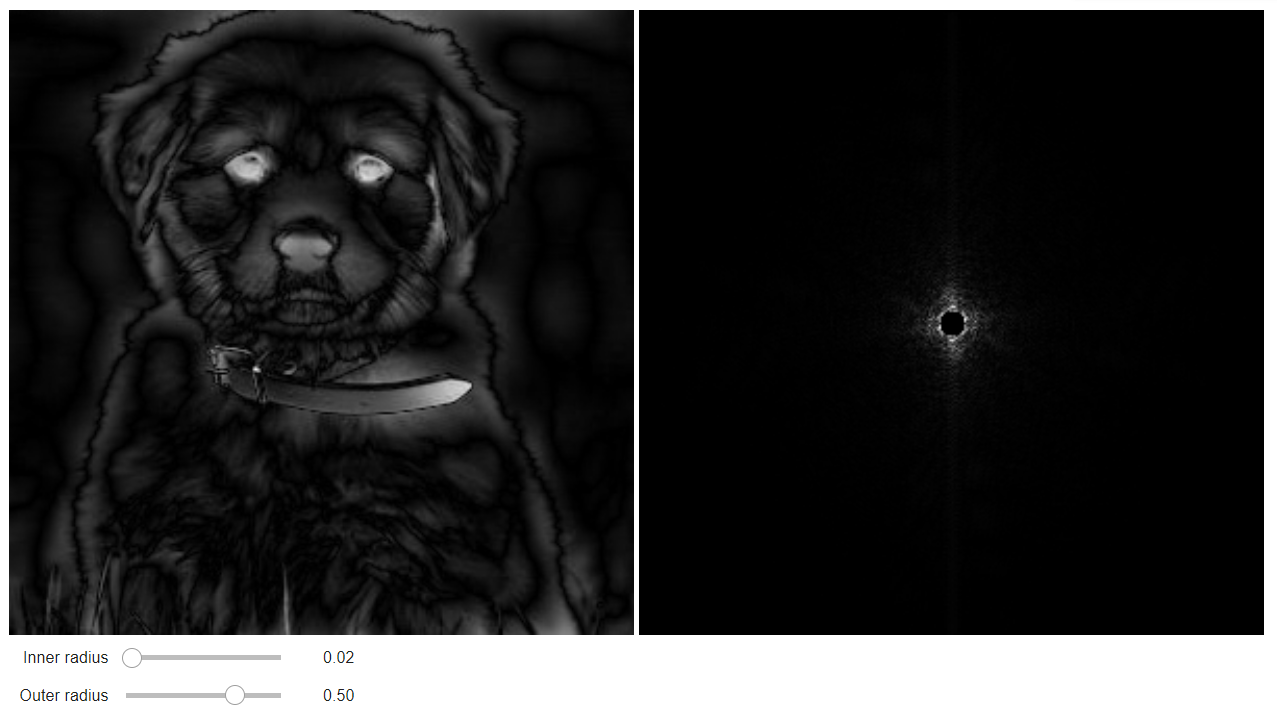
\includegraphics[width=0.75\textwidth]{ex23_output}
    \caption{After filter\_frequency() function}
    \label{ex23_output}
\end{figure}


\subsubsection{Kết quả sau khi thực hiện create\_hybrid\_img() function}
\begin{itemize}
    \item Ảnh thu được:
\end{itemize}

\begin{figure}[H]
    \centering
    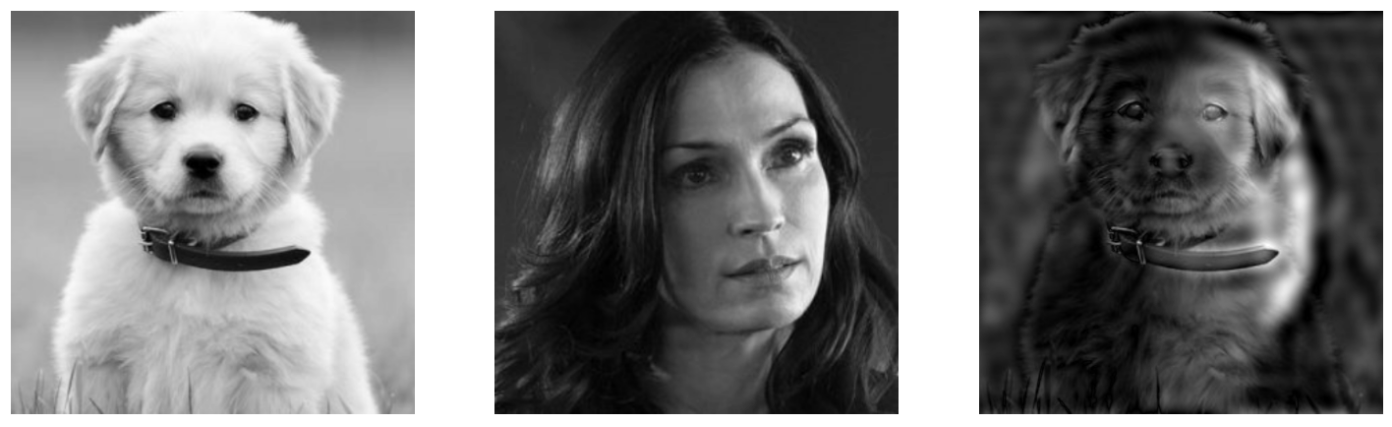
\includegraphics[width=0.75\textwidth]{ex24_output}
    \caption{After create\_hybrid\_img() function}
    \label{ex24_output}
\end{figure}



\end{document}
